% 1987 年全国卷理科第 8 题：y=arccos(cos x) 在 [-pi/2,pi/2] 上的四个图象选项
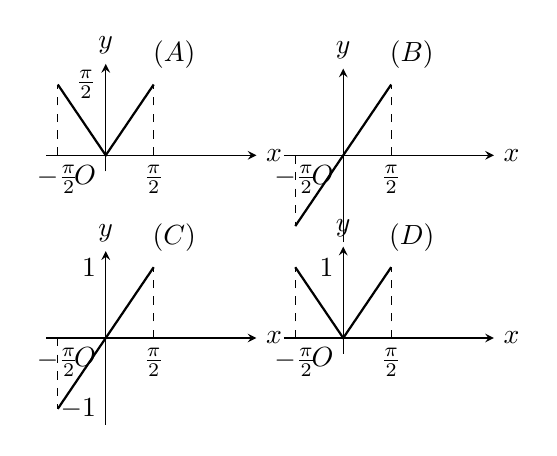
\begin{tikzpicture}[scale=0.58,>=stealth]
  \node at (1.5,2.2) {$(A)$};
  \draw[->] (-1.3,0)--(3.3,0) node[right] {$x$};
  \draw[->] (0,-0.35)--(0,2.0) node[above] {$y$};
  \draw[thick] (-1.05,1.55)--(0,0)--(1.05,1.55);
  \draw[dashed] (-1.05,0)--(-1.05,1.55) (1.05,0)--(1.05,1.55);
  \node[below] at (-1.05,0) {$-\frac\pi2$};
  \node[below] at (1.05,0) {$\frac\pi2$};
  \node[left] at (0,1.55) {$\frac\pi2$};
  \node[below left] at (0,0) {$O$};

  \begin{scope}[xshift=5.2cm]
    \node at (1.5,2.2) {$(B)$};
    \draw[->] (-1.3,0)--(3.3,0) node[right] {$x$};
    \draw[->] (0,-1.9)--(0,1.9) node[above] {$y$};
    \draw[thick] (-1.05,-1.55)--(1.05,1.55);
    \draw[dashed] (-1.05,0)--(-1.05,-1.55) (1.05,0)--(1.05,1.55);
    \node[below] at (-1.05,0) {$-\frac\pi2$};
    \node[below] at (1.05,0) {$\frac\pi2$};
    \node[below left] at (0,0) {$O$};
  \end{scope}

  \begin{scope}[yshift=-4.0cm]
    \node at (1.5,2.2) {$(C)$};
    \draw[->] (-1.3,0)--(3.3,0) node[right] {$x$};
    \draw[->] (0,-1.9)--(0,1.9) node[above] {$y$};
    \draw[thick] (-1.05,-1.55)--(1.05,1.55);
    \draw[dashed] (-1.05,0)--(-1.05,-1.55) (1.05,0)--(1.05,1.55);
    \node[below] at (-1.05,0) {$-\frac\pi2$};
    \node[below] at (1.05,0) {$\frac\pi2$};
    \node[left] at (0,1.55) {$1$};
    \node[left] at (0,-1.55) {$-1$};
    \node[below left] at (0,0) {$O$};
  \end{scope}

  \begin{scope}[xshift=5.2cm,yshift=-4.0cm]
    \node at (1.5,2.2) {$(D)$};
    \draw[->] (-1.3,0)--(3.3,0) node[right] {$x$};
    \draw[->] (0,-0.35)--(0,2.0) node[above] {$y$};
    \draw[thick] (-1.05,1.55)--(0,0)--(1.05,1.55);
    \draw[dashed] (-1.05,0)--(-1.05,1.55) (1.05,0)--(1.05,1.55);
    \node[below] at (-1.05,0) {$-\frac\pi2$};
    \node[below] at (1.05,0) {$\frac\pi2$};
    \node[left] at (0,1.55) {$1$};
    \node[below left] at (0,0) {$O$};
  \end{scope}
\end{tikzpicture}
